\documentclass{article}
\usepackage[utf8]{inputenc}
\usepackage{graphicx}
\usepackage{apuntes-ucppm}
\usepackage{fancyhdr}
\usepackage{amsmath}
\usepackage{bookmark}
\usepackage[a4paper, margin=1.25in]{geometry}
\usepackage{tikz}
\usepackage{calc}

\usetikzlibrary{positioning,matrix, patterns,decorations.pathreplacing}

\title{Vectores C++ STL}
\logo{logo.png}
\author{Jorge Hernández Palop}

\tikzset{
  pics/array/.style 2 args={
    code = {
        \foreach \x [count=\xi, evaluate=\x as \sep using #2*\xi] in #1 {
            \node [draw, minimum size=#2 cm] at (\sep, 0) {\x};
        }
    }
  },
  pics/borderless array/.style 2 args={
    code = {
        \foreach \x [count=\xi, evaluate=\x as \sep using #2*\xi] in #1 {
            \node [minimum size=#2 cm] at (\sep, 0) {\x};
        }
    }
  }
}

\begin{document}
    \maketitle
    \section{Introducción}
    \subsection{¿Qué es un vector?}

    Un \textbf{vector} es una \textbf{estructura de datos} que nos permite guardar \textbf{elementos de un mismo
    tipo} de manera \textbf{secuencial}. Es decir es una lista de elementos del mismo tipo. 

    Existen otros mecanismos que nos permiten hacer lo mismo, como los arrays. Pero la principal ventaja
    de los vectores es que podemos \textbf{aumentar y disminuir el tamaño de nuestro vector a lo largo de 
    la ejecución del programa}, algo imposible con los arrays.

    Para poder usar los vectores deberemos de \textbf{importalos de la librería estándar de C++} 
    por medio del siguiente comando \texttt{\#include <vector>}.
    
    \begin{figure}[h]
        \centering
        \begin{tikzpicture}
            \def\mylist{3, 4, 2, -1, 4, 1, 2, 3}
            \def\size{0.8}
            \draw pic (A)  {array={\mylist}{\size}};
            \draw node (B) [left = -1em of A]  {$v=$};
        \end{tikzpicture}
        \caption{Representación gráfica de un vector \texttt{v} de tamaño 8  de tipo \texttt{int}}
    \end{figure}

    \subsection{¿Cómo acceder a los elementos de un vector?}


    Para acceder a cada elemento de un vector se debe usar un \textbf{indice} que corresponde con la \textbf{posición
    del elemento} dentro del vector. En la mayoría de lenguajes de programación el indice \textbf{comienza en 0}
    y C++ no es la excepción.
    
    Para acceder a los elementos indicaremos el nombre del vector y el indice entre paréntesis,
    por ejemplo, \texttt{miVector[0]}.

    \textbf{IMPORTANTE:} Solo podemos usar indices que se encuentren en el rango $[0, \text{tamaño vector})$.
    Si tratamos de acceder elementos fuera del tamaño del vector lo más posible es que el programa explote.

    \begin{figure}[h]
        \centering
        \begin{tikzpicture}
            \def\mylist{3, 4, 2, -1, 4, 1, 2, 3}
            \def\index{$v[0]$, $v[1]$, $v[2]$, $v[3]$, $v[4]$, $v[5]$, $v[6]$, $v[7]$}
            \def\size{0.8}

            
            \draw  pic (A) {array={\mylist}{\size}};
            \draw node (B) [left = -1em of A]  {$v=$};
            \draw pic (C) [below = 1em of A] {borderless array={\index}{\size}};
            \end{tikzpicture}
        \caption{Indices del vector $v$}
    \end{figure}

    \subsection{¿Cómo se crea un vector?}

    Existen varias maneras de crear o inicializar un vector. Estas son algunas, la primera es usando el constructor
    por defecto. De esta manera creamos un vector de tamaño 0 con el tipo (\texttt{int, string, long long...}) que especifiquemos.
    $$\texttt{vector<tipoElementos> miVector;}$$

    La segunda manera es especificando el tamaño del vector antes de crearlo, de esta manera nos aseguraremos que el vector
    tenga un tamaño minimo antes de operar con él. Todos los elementos del vector pasarán a tener un valor por defecto
    que dependerá del tipo del vector, en el caso de los tipos númericos este valor será 0.

    $$\texttt{vector<tipoElementos> miVector(tamanoVector);}$$

    La tercera forma de crearlo es indicando un valor por defecto al vector además del tamaño. El resultado es el mismo
    que de la manera anterior, lo único que cambia es el valor por defecto con el que comienza cada elemento. 

    $$\texttt{vector<tipoElementos> miVector(tamanoVector, valorPorDefecto);}$$

    La última manera que se usa en programación competitiva es mediante inicialización de listas. Le pasamos una serie
    de elementos entre llaves al vector. El vector resultante tendra exactamente el tamaño de la lista que le hemos
    introducido y los elementos en el orden en el que se encontraban en la lista.

    $$\texttt{vector<tipoElementos> miVector \{elemento0, elemento1, ..., elementoN-1\};}$$

    \subsubsection{Ejemplos}

    \begin{figure}[h]
        \centering
        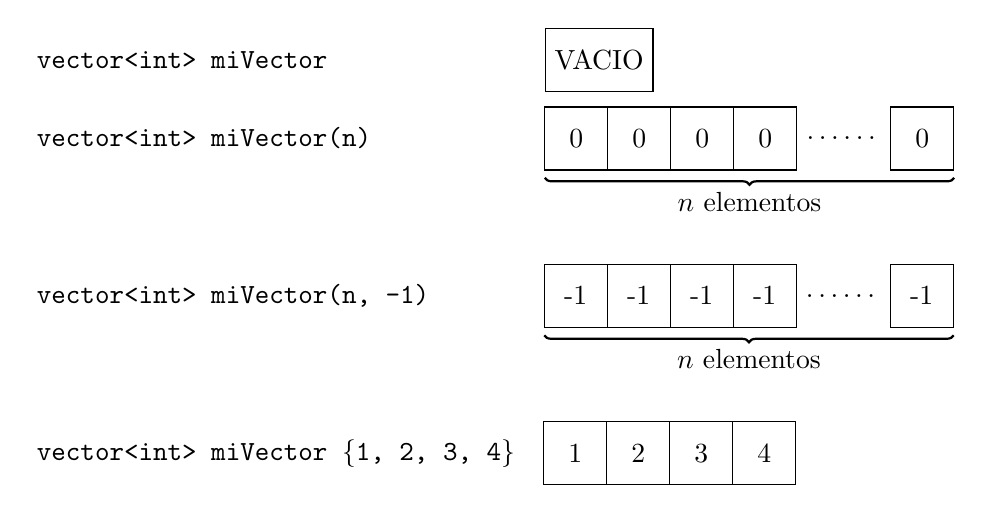
\begin{tikzpicture}
            % Defecto
            \draw node (vector1N) {\texttt{vector<int> miVector}};
            \draw node[draw, minimum size = 0.8cm, local bounding box=vector1, right = 7.5em of vector1N] {VACIO};
            
            \draw node[below = of vector1N.west, anchor=west] (vector2N) {\texttt{vector<int> miVector(n)}};
            \draw pic[below = of vector1.west, anchor=east, local bounding box=vector2] {array={{0, 0 , 0, 0}}{0.8}};
            \draw node[right = 0 of vector2] (vector2D) {\dots\dots};
            \draw node[draw, right = 0em of vector2D, minimum size = 0.8cm] (vector2M) {0};
            \draw [
            thick,
            decoration={
                brace,
                mirror,
                raise=0.5cm
            },
            decorate 
            ] (vector2.west) -- (vector2M.east) node [pos=0.5,anchor=north,yshift=-0.55cm] {$n$ elementos}; 

            \draw node[below = 2 of vector2N.west, anchor=west] (vector3N) {\texttt{vector<int> miVector(n, -1)}};
            \draw pic[below = 2 of vector2.west, anchor=east, local bounding box=vector3] {array={{-1, -1 , -1, -1}}{0.8}};
            \draw node[right = 0 of vector3] (vector3D) {\dots\dots};
            \draw node[draw, right = 0em of vector3D, minimum size = 0.8cm] (vector3M) {-1};
            \draw [
            thick,
            decoration={
                brace,
                mirror,
                raise=0.5cm
            },
            decorate 
            ] (vector3.west) -- (vector3M.east) node [pos=0.5,anchor=north,yshift=-0.55cm] {$n$ elementos}; 

            \draw node[below = 2 of vector3N.west, anchor=west] (vector4N) {\texttt{vector<int> miVector \{1, 2, 3, 4\}}};
            \draw pic[below = 2 of vector3.west, anchor=east, local bounding box=vector4] {array={{1, 2, 3, 4}}{0.8}};

        \end{tikzpicture}
        \caption{Distintos tipos de inicialización de vectores}
    \end{figure}

    \subsection{Notas Extras}

    \textit{En muchos problemas nos darán el tamaño del vector antes de decirnos sus elementos, en estos casos crear un 
    vector vacio de tamaño n es nuestra mejor opción ya aunque como veremos más adelante aumentar el tamaño del vector mientras
    insertamos elementos en un vector es 'rápido', esto supone un coste extra y hará que nuestro programa corra más rápido. 
    Por lo tanto el 75\% de las veces  va a ser mejor inicializar un vector con un tamaño n, antes que ir insertando elementos poco a poco. }
    \pagebreak
    \section{Operaciones básicas}

    Ya hemos visto algunas operaciones básicas de los vectores, cómo crearlos y cómo acceder a sus elementos. Ahora veremos
    otras operaciones igual de importantes.

    \subsection{Leer vectores de la entrada estándar}

    Hemos visto que podemos inicializar el vector con valores por defecto o por medio de una lista. Sin embargo queremos
    poder cambiar esos valores según la entrada del problema para ello veremos dos maneras.

    La primera manera es asegurándonos de que tenemos el espacio suficiente para todos los elementos dentro del vector
    y por medio de un bucle ir leyendo de la entrada e ir rellenando el vector.

    \begin{codelisting}{Leer un vector de la entrada estándar 1}
int numeroElementos;
cin >> numeroElementos;

vector<int> v(numeroElementos);
for(int i = 0; i < numeroElementos; i++) {
    // Forma 1
    int x; 
    cin >> x; 
    v[i] = x;

    // Forma 2
    cin >> v[i];
}
    \end{codelisting}

    Otra formas menos recomendable, es inicializar un vector vacio e ir insertando elementos detrás por medio del método
    \texttt{push\_back}. Si hacemos \texttt{v.push\_back(elemento)} aumentaremos el tamaño del vector en uno e 
    insertaremos el nuevo elemento al final.

    \begin{codelisting}{Leer un vector de la entrada estándar 2}
    int numeroElementos;
    cin >> numeroElementos;
    
    vector<int> v;
    for(int i = 0; i < numeroElementos; i++) {
        int x; 
        cin >> x; 
        v.push_back(x);
    }
    \end{codelisting}

    \subsection{Insertar elementos}

    Existen dos opciones para insertar nuevos elementos dentro del vector. La primera opción es usar \texttt{push\_back},
    este método es muy rápido (tiene un coste amortizado de $\mathcal{O}(1)$). Se usa así \texttt{miVector.push\_back(elemento)} . Lo que hace es añadir el elemento al final 
    del vector. El segundo método, es el método \texttt{insert} que nos permite seleccionar en que posición colocar el
    nuevo elemento, antes de ser colocado todos los elementos a la derecha se ruedan a una posición para poder hacer hueco
    al nuevo elemento. Este método es mucho más lento sobretodo cuando la posición sea cercana a 0 (tiene un coste de $\mathcal{O}(n)$). 
    Se usa así \texttt{miVector.insert(elemento, posición)}.

    \begin{figure}[h]
        \centering
        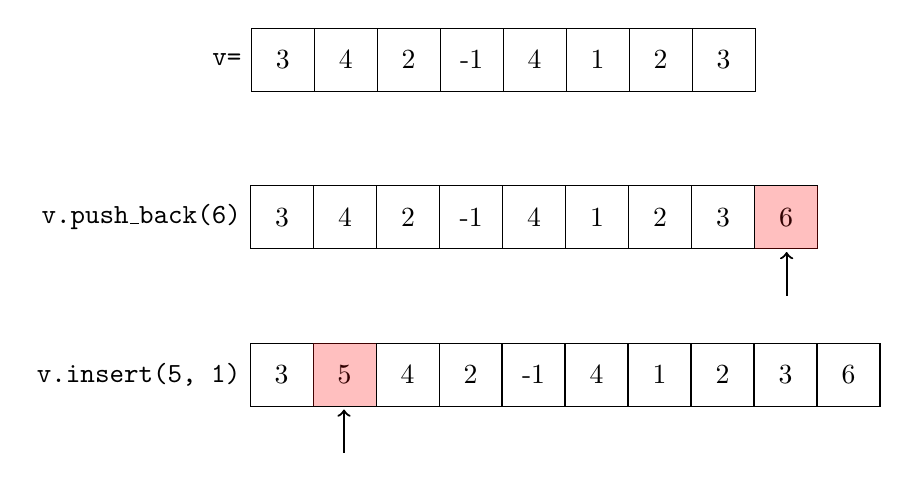
\begin{tikzpicture}
            \def\mylist{3, 4, 2, -1, 4, 1, 2, 3}
            \def\size{0.8}
            \draw pic [local bounding box=A] {array={\mylist}{\size}};
            \draw node (B) [left = 0em of A]  {\texttt{v=}};

            \def\mylist{3, 4, 2, -1, 4, 1, 2, 3, 6}
            \draw pic [below = 2 of A.west, anchor=east, local bounding box=C] {array={\mylist}{\size}};
            \draw node (D) [right = -0.8cm of C, minimum size = \size cm, fill=red, opacity=0.25] {6};
            \draw node (B) [left = 0em of C]  {\texttt{v.push\_back(6)}};
            \draw[thick,<-,shorten <=1pt] (D) -- +(-90:1cm);

            \def\mylist{3, 5, 4, 2, -1, 4, 1, 2, 3, 6}
            \draw pic [below = 2 of C.west, anchor=east, local bounding box=E] {array={\mylist}{\size}};
            \draw node (F) [left = -1.6cm of E, minimum size = \size cm, fill=red, opacity=0.25] {5};
            \draw node (G) [left = 0em of E]  {\texttt{v.insert(5, 1)}};
            \draw[thick,<-,shorten <=1pt] (F) -- +(-90:1cm);
        \end{tikzpicture}
        \caption{Ejemplo de inserción de elementos con \texttt{push\_back} e \texttt{insert}}
    \end{figure}

    \begin{codelisting}{Inserción de elementos}
int n = 4;        
vector<int> v(n);
for(int i = 0; i < numeroElementos; i++) {
    v[i] = i;
}
// v = {0, 1, 2, 3};

v.push_back(6); // v = {0, 1, 2, 3, 6};

v.insert(-1, 1); // v = {0, -1, 1, 2, 3, 6};
        \end{codelisting}

\end{document}

    